\documentclass{article}

\usepackage[a4paper,margin=2cm]{geometry}
\usepackage{color, soul}
\usepackage{titlesec}
\usepackage{enumitem}
\usepackage{pdfpages}
\usepackage{multicol}
\usepackage{fancyvrb}
\usepackage{float}

\title{SWEN30006 Assignment 2 - Report}
\date{\today}
\author{Workshop 09, Team 02\\Lucas Fern \& Cameron Maddern}

\begin{document}
\maketitle
This project required changes to be made to an existing Cribbage card game trainer system to add scoring and logging functionality. These additions were made with the use of a variety of design patterns in order to have minimum impact on the existing code, and therefore reduce coupling between existing classes and classes added for the new functionality.\\[2mm]
This report will discuss the changes which have been made, provide justification for the design patterns used, \hl{and argue in favour of these design patterns over the use of others where appropriate.} The additional classes will be covered first, then how these additional classes were integrated into the existing system.\\[2mm]
A class diagram of the updated design is included at the end of the report and will be relevant to visualise all changes to the system.

\section{Cribbage Observers}
In an effort to minimise coupling between added classes and maximise cohesion within them, a \verb|CribbageObserver| interface was implemented. This allowed classes to subscribe to various events of the Cribbage game, and respond with unique actions. This required the addition of a list of subscribers in the main \verb|Cribbage| class, as well as a method to register new subscribers.

\subsection{Cribbage Events}
\label{sec: crib events}
Now that a publish-subscribe pattern is implemented it must be decided when events are broadcast to the subscribers. There are a variety of events in the game of Cribbage, and it was decided that all events which relate to the logging and scoring functionality will be broadcast to the subscribers. This allows - for example - the logging functionality for the \verb|deal| to be implemented by an observer responding to a \verb|Deal| event. The various subscribers to Cribbage Events are discussed further in Section \ref{sec: crib subscribers}.\\[2mm]
The complete list of \verb|CribbageEvent|s implemented appears on the right side of the class diagram, and their functionality is briefly summarised below:
\begin{multicols}{2}
    \begin{itemize}
        \item \verb|SetSeed|\\[2mm]
        Subscribers are notified of this event when the game's seed is set from the \verb|cribbage.properties| file. The event contains the random seed which was chosen.
        \item \verb|InitPlayer|\\[2mm]
        This event is broadcast when the players of the game are initialised and assigned a number. This provides subscribers with information about the player type which has been initialised (\textit{eg.} \verb|cribbage.RandomPlayer|) and their number.
        \item \verb|Discard|\\[2mm]
        This event is created once for each player each game, when the player has selected which cards to discard. It provides observers with the players number, and a \verb|jcardgame.Hand| object containing the cards they selected for discarding.
        \item \verb|PlayStarter|\\[2mm]
        The \verb|PlayStarter| event is published once per game when the starter card is selected, and provides the starter card as a \verb|jcardgame.Card|.
        \item \verb|Play|\\[2mm]
        This event is raised on every turn of the game, when a player selects the card they wish to play. It contains the player's number, the card they played, and the total face value of the current board after adding this card.
        \item \verb|Show|\\[2mm]
        The \verb|Show| event occurs at the end of the game when play has ceased and players are showing card combinations from their hands to be scored. This event contains information about the player's number, the starter card, and the cards that they are showing to be scored.
    \end{itemize}
\end{multicols}
\begin{itemize}
    \item \verb|Score|\\[2mm]
    The \verb|Score| event is a special type of event raised by the Cribbage Scorer in response to other events, it occurs whenever a player's score is incremented, and contains data on the amount of points scored, their total score, and the type of score achieved. This will be discussed further in \ref{sec: crib scorer}.
\end{itemize}
Each of these events also overrides the default \verb|toString()| method. Their implementation of the method returns a \verb|String|, formatted as required for the logging functionality. This will be discussed further in Section \ref{sec: crib logger}


\subsection{Cribbage Subscribers}
\label{sec: crib subscribers}
Subscribers are classes which implement the \verb|CribbageObserver| interface and register with the \verb|Cribbage| class to be notified of game events. Their creation and registration is done inside the \verb|Cribbage| class since currently the only subscribers are the Logger and Scorer, \hl{which was not complex enough to justify their creation in an external factory.}
\subsubsection{Cribbage Scorer}
\label{sec: crib scorer}
The \verb|CribbageScorer| class, is cohesively responsible for handling all scoring events in the Cribbage game. \verb|CribbageScorer| subscribes to the \verb|Cribbage| class and its \verb|update()| method is called whenever an event (defined in Section \ref{sec: crib events}) occurs.\\[2mm]

On creation of the \verb|CribbageScorer|, any method of scoring must subscribe to the \verb|CribbageScorer|, imilar to the \verb|CribbageObserver| interface. These methods all implement the \verb|ScoringEvent| interface with the 2 methods:
\begin{figure}[H]
\centering
\begin{BVerbatim}
int scoreForPlay(Hand cardSet, int playerScore, int playerNum);
int scoreForShow(Hand cardSet, int playerScore, int playerNum);
\end{BVerbatim}
\end{figure}

This allows for simple extensibility as any new method of scoring must only subscribe to the \verb|CribbageScorer| class and implement the \verb|ScoringEvent| interface.\\[2mm]

The distinction between the two methods \verb|int scoreForPlay()| and \verb|int scoreForShow()| allows for variations in scoring to be easily implemented. For example, if a variation did not include flushes then this would be implemented by not subscribing the \verb|HandleFlushes| class to \verb|CribbageScorer|, or if a variation were not to include runs in the \verb|show| phase of the game, then \verb|int scoreForShow()| in the \verb|Handleruns| class could simply return the \verb|playerScore| that was passed in.\\[2mm]


On notification of any event, the cribbage scorer determines any cards that need to be stored as having been played, and notifies scorers to determine if a scoring situation has occurred.
\subsubsection{Cribbage Logger}
\label{sec: crib logger}
The \verb|CribbageLogger| class \hl{[singleton?]}, which appears in the bottom left of the class diagram, is cohesively responsible for all of the logging functionality of the game. As a subscriber to the \verb|Cribbage| class, the logger's \verb|update()| method is called whenever an event (defined in Section \ref{sec: crib events}) occurs. The event is passed through to the class in this method call.\\[2mm]
On notification of any event, the cribbage logger calls the event's \verb|toString()| method, yielding the information required for logging, and uses a \verb|BufferedWriter| to write this to \verb|cribbage.log|. Taking a \verb|Play| event for example, the contents and respective string representation might be:
\begin{figure}[H]
\centering
\begin{BVerbatim}
examplePlay = {                              |
    eventId: "play",  [String]               |
    playerId: "P0",   [String]               |      String representation:
    totalPoints: 23,  [int]                  |      "play,P0,23,KH"
    card: KH          [jcardgame.Card]       |  
}                                            |
\end{BVerbatim}
\end{figure}
\noindent This highly cohesive design, enabled by the observer pattern, is all that is required for the logging functionality.

\section{Changes to Existing Classes}
Changing existing classes was avoided as much as possible when adding the new functionality to reduce the possibility of bloated classes, and reduce coupling with new classes. This section will provide justification for the few changes which were made to the existing classes despite these considerations.
\subsection{Cribbage}
The \verb|Cribbage| class is where most of the changes to existing classes were made. The changes made here are:
\begin{itemize}
    \item \textbf{Adding the Subscriber Functionality}\\[2mm]
    Since the majority of additions to the system were made by implementing the observer pattern, an attribute had to be added to the \verb|Cribbage| class to store the list of classes which subscribe to the events. A method to register subscribers was also added so that the \verb|CribbageScorer| and \verb|CribbageLogger| could register themselves to be notified.
    \item \textbf{The Registration of Subscribers}\\[2mm]
    Since they are separate classes, the \verb|CribbageScorer| and \verb|CribbageLogger| must be instantiated at the beginning of the game, and registered as subscribers to the \verb|Cribbage| class. \hl{It was decided that this was an appropriate amount of code (2 lines) to add to the cribbage class, as opposed to creating a factory to instantiate these classes (which would itself need to be initialised on start-up.)}
    \item \textbf{Privacy / Visibility Changes}\\[2mm] 
    To support the functionality of the new system, it was sensible to change the privacy of certain methods. The most significant change was to each of the 4 \verb|canonical()| methods, which were \verb|private| instance methods in the original design, and have been changed to \verb|public| \verb|static| methods. They were able to be converted to \verb|static| since the conversion of \verb|jcardgame| objects to \verb|String|s did not strictly require any attributes of the \verb|Cribbage| instance.\\[2mm]
    This change was made to support the logging functionality, since the log file contains canonical representations of the cards and hands, and the \verb|String|ification of the \verb|jcardgame| objects occurs in the \verb|toString()| methods of each of the \verb|CribbageEvent|s. Considering the alternative would be to pass string representations as well as the original \verb|jcardgame| objects around with each event; and the fact that there is no clear downside to this change, this was an obvious choice.
\end{itemize}

% 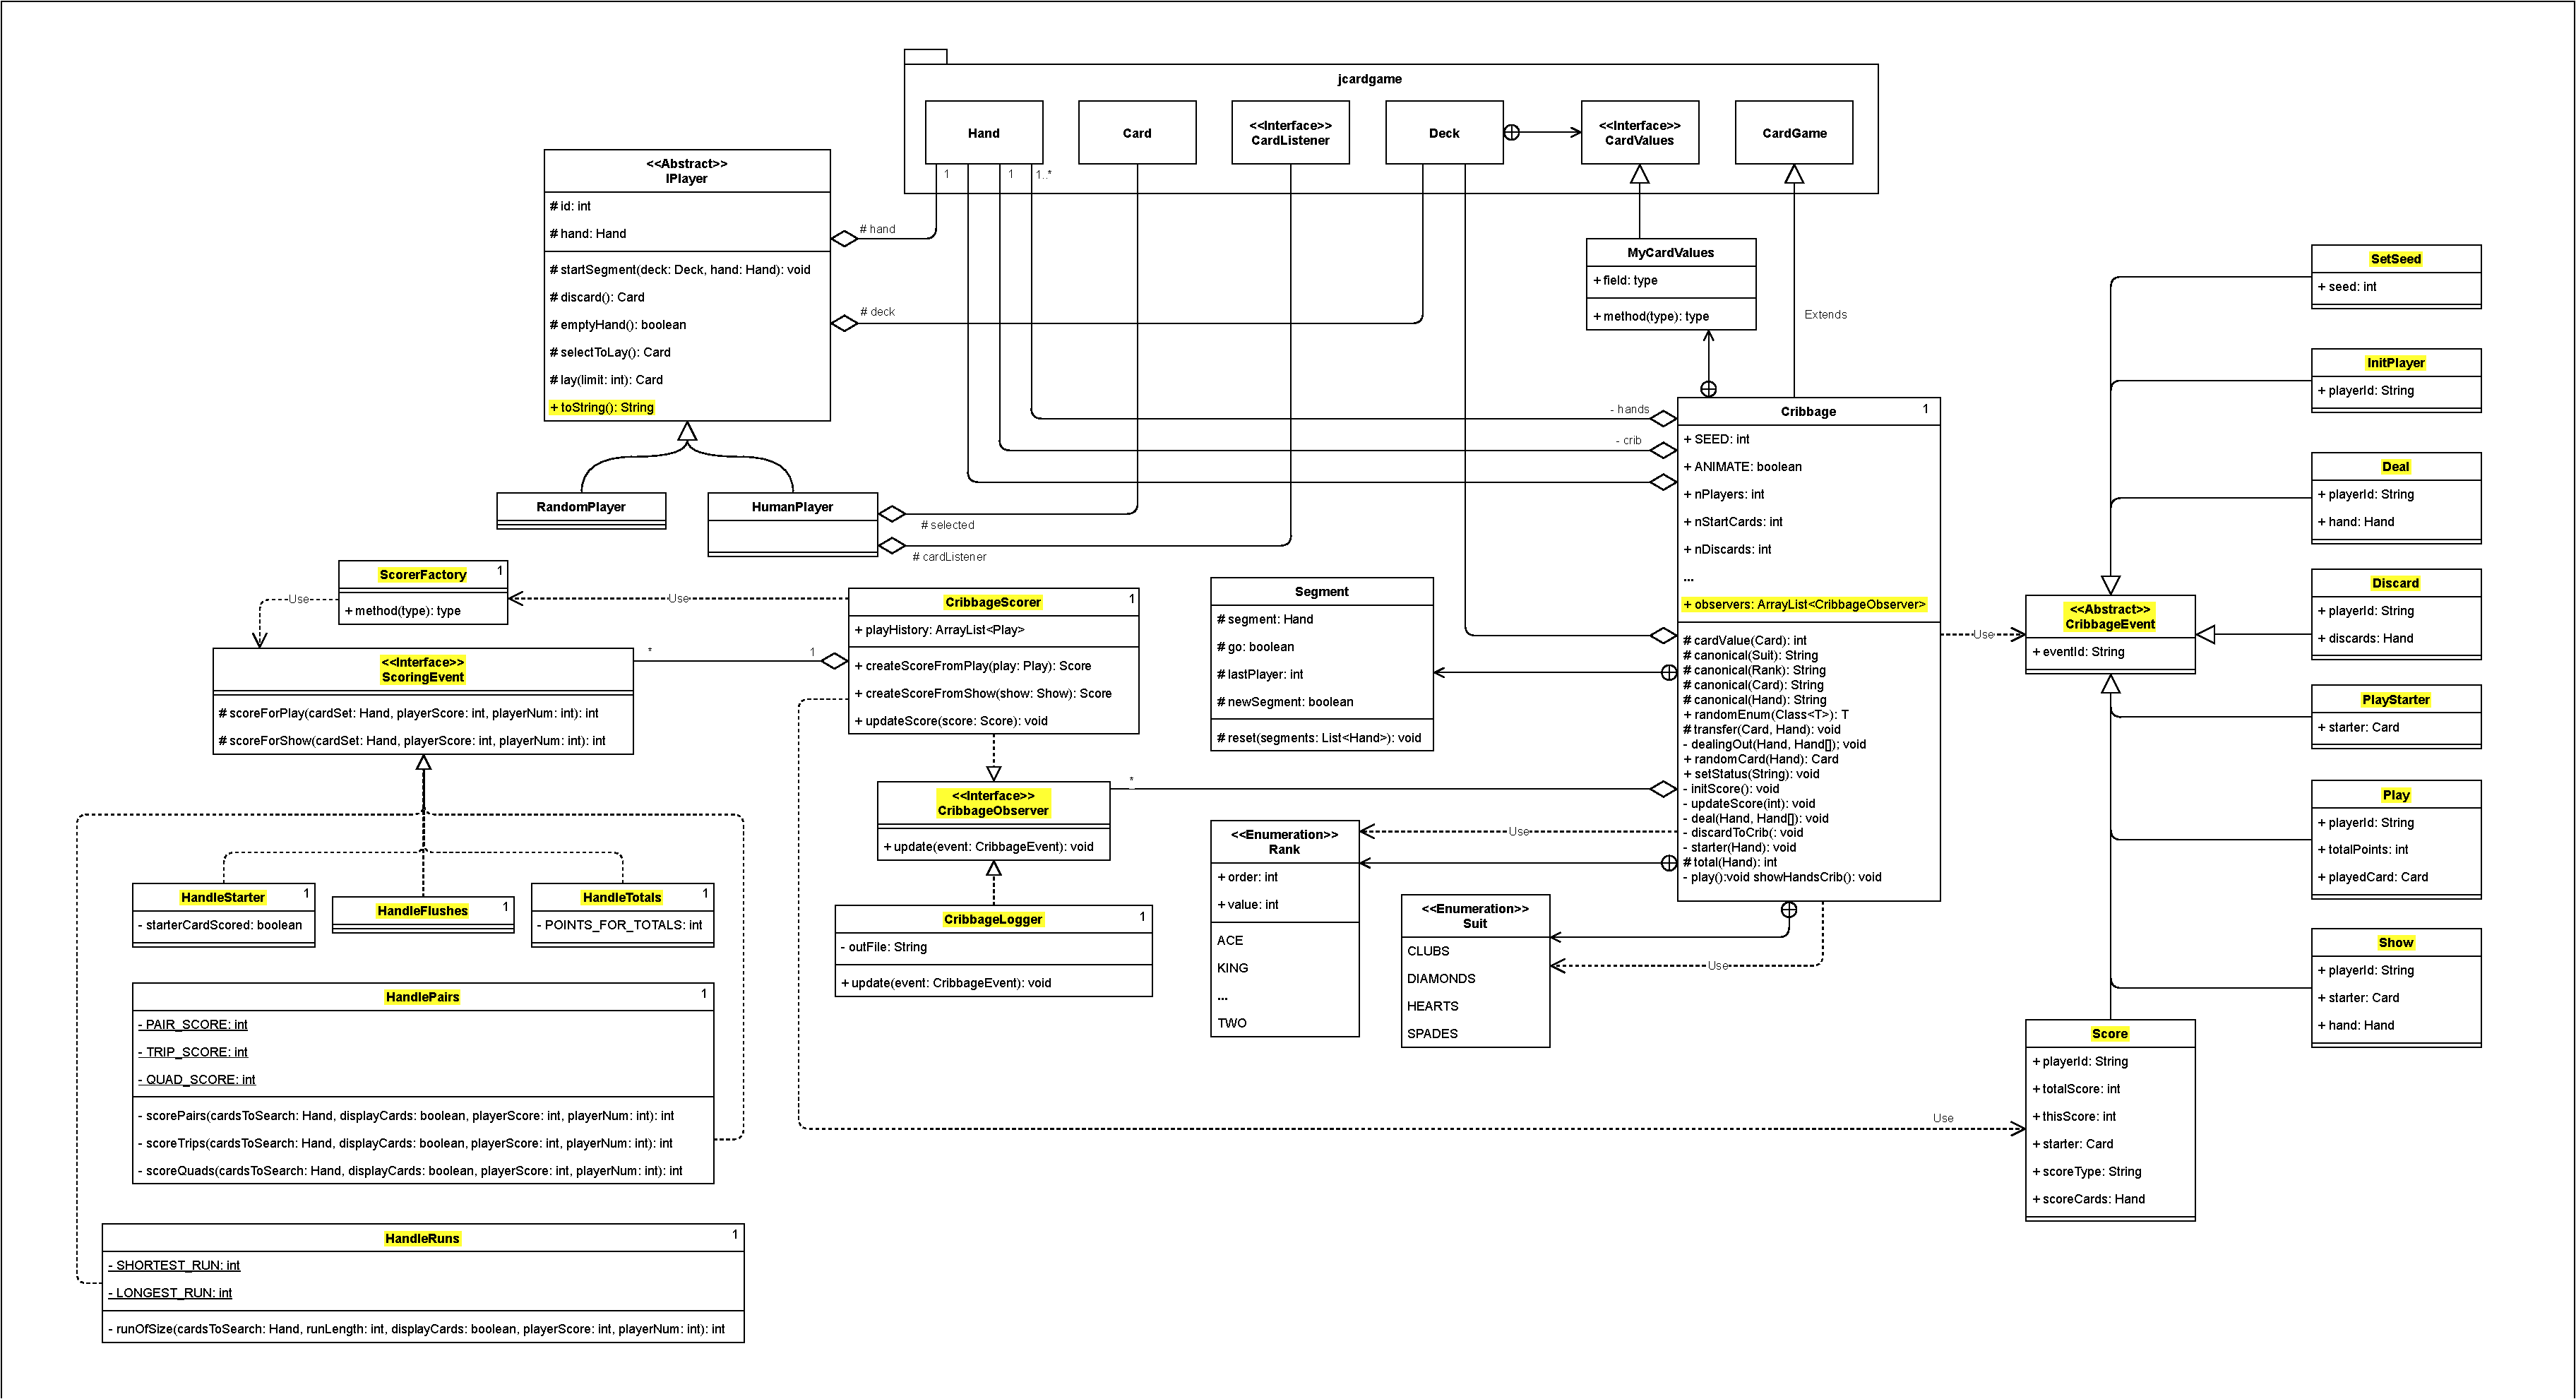
\includepdf[pages=-, fitpaper=true]{design-class-diag.pdf}
\end{document}
